\documentclass{article}
\usepackage[utf8]{inputenc}
\usepackage[spanish]{babel}
\usepackage{verbatim} % comentarios
\title{Proyecto Matlab}


\date{June 2018}
\usepackage{natbib}
\usepackage{graphicx}
\begin{document}

\maketitle
\begin{center}
David Silva

Norman Saldaña 19

Hector Espino 21

Daniel Pineda 20
\end{center}
\section{Introducción}
Este proyecto, se basa en datos estadísticos extraídos directamente de la página del Sistema de Transporte Colectivo Metro de la Ciudad de México y no pretende hacer mal uso de esta información.

\section{Desarrollo}
\subsection{¿Qué es la inteligencia Artificial?}
Existen varias formas de definir la inteligencia artificial, dependiendo el contexto como \textit{human performance} o \textit{racionality} (entendiendo por racionalidad al proceso de hacer las <<cosas correctas>> dependiendo de lo que nosotros entendemos como <<correcto>>). Entre los enfoques mencionados existe un tipo de enfrentamiento, sin en¿mbargo ambos se complementan. Por un lado, el enfoque centrado en el comportamiento humano, debe ser una ciencia empírica, que influya hipótesis y confirmaciones mediante experimentos. El enfoque racional, por otro lado, implica una combinación de matemáticas e ingeniería.

Varios han tratado de definir a la inteligencia artificial desde hace años, uno de los cuales se cita a continuación <<El estudio de las facultades mentales mediante el uso de modelos computacionales>> (Charniak y McDermott, 1985).

Existe una prueba llamada la prueba de Touring, la cual se diseñó para proporcionar una definición operacional y satisfactoria de la inteligenica. Para que una computadora pueda pasar la prueba de Touring debe de tener las capacidades de:

\begin{itemize}
    \item Procesamiento de lenguaje natural que permita comunicarse satisfactoriamente
    \item Representación del conocimiento para almacenar lo que conoce o siente.
    \item Razonamiento automático para utilizar la información almacenada para responder a preguntas y extraer nuevas conclusiones.
    \item Aprendizaje automático para adaptarse a nuevas circunstancias y para detectar y extrapolar patrones.
\end{itemize}

\subsection{Enfoques de la inteligencia artificial}

Ahora bien, existen tres principales enfoques de la inteligencia artificial: \textbf{cognitivo, <<leyes del pensamiento>>, agentes racionales}. Se hablará un poco de cada uno de estos para entenderlos mejor, a grandes rasgos, el \textit{modelo cognitivo} 

\subsubsection{Actuar como huamno: Enfoque cognitivo}

Para este enfoque es necesario \textit{adentrarse} en el funcionamiento de las mentes humanas y, para ello, existen dos maneras de hacerlo; introspección (captar los pensamientos conforme se van generando) y mediante experimentos psicológicos. Teniendo claro cómo funciona la mente humana, entonces se podrá expresar en forma de un programa de computadora. Hay evidencia de que algunos de los mecanismos del programa se pueden comparar con los de los seres humanos si éstos presentan las mismos datos de entrada/salida y similares tiempos de reacción. En el campo interdisciplinario de la ciencia cognitiva convergen modelos computacionales de IA y técnicas experimentales de psicología intentando elaborar teorías precisas y verificables sobre el funcionamiento de la mente humana.

La auténtica ciencia cognitiva se fundamenta en la investigación experimental en humanos y animales y, puesto que para la IA sólo se dispone de una computadora para experimentar, solía haber cierta confusión entre las distintas aproximaciones:  un autor podría argumentar que un algoritmo resolvía adecuadamente una tarea y que por tanto era un buen modelo de representación humana, o viceversa. Actualmente, se hace diferencia entre las dos reivindicaciones; esta distinción ha permitido que ambas disciplinas, IA y ciencia cognitiva, se desarrollen más rápidamente. Los dos campos continúan alimentándose entre sí, especialmente en las áreas de la visión y el lenguaje natural. En particular, el campo de la visión ha avanzado recientemente con la ayuda de una propuesta integrada que tiene en cuenta la evidencia neurofisiológica y los modelos computacionales.

\subsubsection{Pensamiento racional: el enfoque de las <<leyes del pensamiento>>}

Uno de los primeros en intentar codificar la <<manera corracta de pensar>> fue Aristóteles. Sus silogismos son esquemas de estructuras de argumentación mediante las que siempre se llega a conlusiones correctas. Por ello, la tradición \textbf{logista} dentro del campo de la inteligencia artifical trata de construir sistemas inteligentes a partir de programas que, en principio, tienen que resolver cualquier problema resoluble descrito en notación lógica.

Las desventajas que tiene este modelo son que no es fácil transformar conocimiento informal y expresarlo en los términos formales que requieren de notación lógica, particularmente cuando el conocimiento que se tiene es inferior al 100 por 100. Otro punto es la gran diferencia entre resolver un problema «en principio» y hacerlo en la práctica. Estos obstáculos están presentes en todo intento de construir sistemas de razonamiento computacional pero surgieron por vez primera en la tradición lógica.

\subsubsection{Actuar de forma racional: el enfoque del agente racional}

Para este enfoque es primordial conocer dos coneptos: \textbf{agente} y \textbf{agente racional}. Entendiéndose por el primero algo que actúa, que hace. Un agente racional, en cambio, es aquél que actúa tratando de lograr el mejor resultado, o cuando no hay certidumbre, el mejor resultado esperado.

 el estudiar la IA desde el enfoque del diseño de un agente racional ofrece al menos dos ventajas. La primera es más general que el enfoque que proporcionan las «leyes del pensamiento», dado que el efectuar inferencias correctas es sólo uno de los mecanismos existentes para garantizar la racionalidad. La segunda es más afín a la forma en la que se ha producido el avance científico que los enfoques basados en la conducta o pensamiento humano, porque la norma de la racionalidad está claramente definida y es de aplicación general.

\subsection{Los fundamentos de la inteligencia artificial}

\subsubsection{Filosofía}

Como ya se había mencionado, Aristóteles (384-322 a.C.)  fue el primero en formular un conjunto preciso de leyes que gobernaban la parte racional de la inteligencia, Desarrolló un sistema ingormal para razonar adecuadamente con silogismos, el cual permitía extraer conclusiones mecánicamente a partir de premisas iniciales. Luego de Aristóteles, vino Ramón Lull (d. 1315), quien tuvo la idea de que el razonamiento útil se podría obtener por medios artificiales.  Thomas Hobbes (15881679) propuso que el razonamiento era como la computación numérica, de forma que <<nosotros sumamos y restamos silenciósamente en nuestros pensamientos>>. Leonardo Da Vinci diseñó una calculadora mecánica. La primera máquina calculadora conocida la hizo el científico alemán Wilhelm Schickard (1592-1635) alrededor de 1623, sin embargo, la Pascalina, construida en 1642 por Blaise Pascal (1623-1662), es la más famosa.

Ahora, en un enfoque que considera a la mente como un sistema físico,  René Descartes (1596-1650) dio la primera discusión clara sobre la distinción entre la mente y la materia y los problemas que surgen. Uno de los problemas de una concepción puramente física de la mente es que parece dejar poco margen de maniobra al libre albedrío. Descartes fue defensor del \textbf{dualismo}. Sostenía que existe una parte de la mente (o del alma/espíritu) que está al margen de la naturaleza, exenta de la influencia de las leyes físicas. Los animales, en cambio, no poseen esta cualidad dual; a ellos se le podría concebir como si se tratasen de máquinas.

Ahora es tiempo de plantearse el problema de establecer las fuentes de ese conocimiento. El movimiento empírico fue inciado por Francis Bacon (1561-1626) en su Novum Organum, se caracteriza por el aforismo de John Locke (1632-1704): <<Nothing is in the understanding, which was not first in the senses>>.  David Hume (1711-1776) propuso en A Treatise of Human Nature (Hume, 1739) lo el principio de \textit{inducción}: las reglas generales se obtienen mediante la exposición a asociaciones repetidas entres sus elementos. Sobre la base de las propuestas de Ludwig Wittgenstein (1889-1951) y Bertrand Russell (1872-1970), el famoso Círculo de Viena, liderado por Rudolf Carnap (1891-1970), desarrolló la doctrina del positivismo lógico (establece que el conocimiento se puede carecetrizar mediante teorías lógicas relacionadas, con sentencias de observación que corresponden a estímulos sensoriales) . La teoría de confirmación de Carnap y Carl Hempel (1905-1997) intenta explicar cómo el conocimiento se obtiene a partir de la experiencia. La primer teoría en mostrar la mente como un proceso computacional se plasma en el libro de Carnap, \textit{The Logical Structure of the World} (1928), donde se define un procedimiento computacional explícito para la extracción de conocimiento a partir de experiencias primarias.

Por último, la relación entre el conocimiento y acción. Para ello, Aristóteles argumentó que las acciones se pueden justificar por la conexión lógica entre los objetivos y el conocimiento de los efectos de las acciones. Su algoritmo se conoce como sistema de planifiación regresivo y se implementó por Newll y Simon con el programa SRGP 2500 años después. 

El análisis basado en objetivos no indica qué hacer cuando varias acciones nos llevan a la consecución del objetivo, o cuando ninguna acción facilita su completa consecución. Antoine Arnauld (1612-1694) describió correctamente una forma cuantitativa para decidir qué acción llevar a cabo en un caso como este. El libro Utilitarianism (Mill, 1863) de John Stuart Mill (1806-1873) propone la idea de un criterio de decisión racional en todos los ámbitos de la actividad humana.

\subsubsection{Matemáticas}

Una vez dichas las ideas más importantes de la IA, se tiene que pasar de ahí a una ciencia formal, por ello es necesario contar con una formulación matemática en tres áreas fundamentales: lógica, computación y probabilidad. 

El concepto de lógica formal comenzó con el trabajo de George Boole (1815-1864) que definió la lógica proposicional o Booleana (Boole, 1847). En 1879, Gottlob Frege (1848-1925) extendió la lógica de Boole para incluir objetos y relaciones, y creó la lógica de primer orden. Alfred Tarski (1902-1983) introdujo una teoría de referencia que enseña cómo relacionar objetos de una lógica con objetos del mundo real. El paso siguiente consistió en definir los límites de lo que se podía hacer con la lógica y la informática. 

Se piensa que el primer algoritmo no trivial es el algoritmo Euclídeo para el cálculo del máximo común divisor. Considerar los algoritmos como objetos en sí mismos se remonta a la época de al-Khowarazmi, un matemático persa del siglo IX, con cuyos escritos también se introdujeron los números arábigos y el álgebra en Europa. Boole, entre otros, presentó algoritmos para llevar a cabo deducciones lógicas. En 1900, David Hilbert (1862-1943) presentó una lista de 23 problemas que acertadamente predijo ocuparían a los matemáticos durante todo ese siglo. 

 Existen algunas funciones de los números enteros que no se pueden representar mediante un algoritmo, es decir no se pueden calcular. Lo anterior llevó a Alan Turing (1912-1954) a tratar de caracterizar exactamente aquellas funciones que sí eran susceptibles de ser caracterizadas.
 
 \subsubsection{Economía}
 
 La ciencia de la economía comenzó en 1776, cuando el filósofo escocés Adam Smith (1723-1790) publicó \textit{An Inquiri into the Nature and Causes of the Wealth of Nations}. Smith fue el primero en tratar el pensamiento económico como una ciencia, con la idea de que las economías pueden concebirse como un conjunto de agentes individuales que intentan maximizar su propio estado de bienestar económico. 
 
La teoría de la decisión (combina la teoría de la probabilidad con la teoría de la utilidad), proporciona un marco completo y formal para la toma de decisiones (económicas o de otra índole) realizadas bajo incertidumbre, esto es, en casos en los que las descripciones probabilísticas capturan adecuadamente la forma en la que se toman las decisiones en el entorno; lo cual es adecuado para <<grandes>> economías  en las que cada agente no necesita prestar atención a las acciones que lleven a cabo el resto de los agentes individualmente. Cuando son <<pequeñas>> economías, la situación se asemeja más a la de un juego: las acciones de un jugador pueden afectar significativamente a la utilidad de otro (tanto positiva como negativamente). Los desarrollos de von Neumann y Morgenstern a partir de la teoríadejuegos(véasetambién Luce y Raiffa, 1957) mostraban el hecho sorprendente de que, en algunos juegos, un agente racional debía actuar de forma aleatoria o, al menos, aleatoria en apariencia con respecto a sus contrincantes.


\subsubsection{Neurociencia}

La Neurociencia es el estudio del sistema neurológico, y en especial del cerebro. El estudio de Paul Broca (1824-1880) sobre la afasia (dificultad para hablar) en pacientes con el cerebro dañado, en 1861, le dio fuerza a este campo y convenció a la sociedad médica de la existencia de áreas localizadas en el cerebro responsables de funciones cognitivas específicas. En particular, mostró que la producción del habla se localizaba en una parte del hemisferio izquierdo; hoy en día conocida como el área de Broca.

En  1873 cuando Camillo Golgi (1843-1926) desarrolló una técnica de coloración que permitió la observación de neuronas individuales en el cerebro (véase la Figura 1.2). Santiago Ramón y Cajal (1852-1934) utilizó esta técnica es sus estudios pioneros sobre la estructura neuronal del cerebro.

En la actualidad se dispone de información sobre la relación existente entre las áreas del cerebro y las partes del cuerpo humano que controlan o de las que reciben impulsos

\subsubsection{Psicología}

Inició con los trabajos del alemán Hermann von Herlmholtz (1821-1894),  y su discípulo Wilhelm Wundt (1832-1920). Helmholtz aplicó el método científico al estudio de la vista humana, y su obra \textit{Handbook of Physiological Optics}, la cual se considera como el <<tratado actual más importante sobre la física y la fisiología de la vista humana>>. El primer laboratorio se abrió en la Universidad de Leipzig por Wundt, se hicieron experimentos controlados de percepción o asociación mientras sometían a introspección sus procesos mentales. Luego evolucionó la psicología hasta convertirse en ciencia pero la subjetividad de los datos de ésta, hizo que fuera difícil para que un investigador contradijera sus propias teorías.

Por otro lado se encuentra el movimiento \textbf{conductista}, lo lideró John Watson. El movimiento rechazó cualquier teoría que involucrara procesos mentales 

\subsubsection{Ingeniería en computación}

\subsubsection{Teoría de control y cibernética}

\subsubsection{Lingüística}
Con la publicación en 1957 de \textit{Verbal Behavior}, de B.F Skinner que abarcaba desde conductista al aprendizaje del lenguaje. El autor Noam Chomsky hizo una revisión del mismo la cual causó gran desinterés en la publicación la decir que ésta no hablaba del tema de la creatividad en el lenguaje, de cómo un infante es capaz de entender y construir oraciones que nunca ha escuchado. La teoría de Chomsky sí explicaba lo anterior y estaba basada en modelos sintácticos remontados al lingüista Panini. A diferencia de las anteriores, poseía el formalismo para permitir su programación.

La lingüística moderna y la IA <<nacieron>>, al mismo tiempo y maduraron juntas, solapándose en un campo híbrido llamado lingüística computacional o procesamiento del lenguaje natural. Surgió un problema del entendimiento del lenguaje muy complejo en 1957. El entendimiento del lenguaje requiere la comprensión de la materia bajo estudio y de su contexto, y no solamente el entendimiento de la estructura de las sentencias. Gran parte de los primeros trabajos de investigación en el área de la representación del conocimiento (el estudio de cómo representar el conocimiento de forma que el computador pueda razonar a partir de dicha representación) estaban vinculados al lenguaje y a la búsqueda de información en el campo del lenguaje, y su base eran las investigaciones realizadas durante décadas en el análisis filosófico del lenguaje.


\subsection{Historia de la inteligencia artificial}

\subsubsection{Génesis de la inteligencia artificial (1943-1955)}

Warren McCulloch y Walter Pitts (1943) han sido reconocidos como los autores del primer trabajo de IA. Partieron de tres fuentes: conocimientos sobre la fisiología básica y funcionamiento de las neuronas en el cerebro, el análisis formal de la lógica proposicional de Russell y Whitehead y la teoría de la computación de Turing. Propusieron un modelo constituido por neuronas artificiales, en el que cada una de ellas se caracterizaba por estar <<activada>> o <<desactivada>>; la <<activación>> se daba como respuesta a la estimulación producida por una cantidad suficiente de neuronas vecinas. El estado de una neurona se veía como «equivalente, de hecho, a una proposición con unos estímulos adecuados». Mostraron, por ejemplo, que cualquier función de cómputo podría calcularse mediante alguna red de neuronas interconectadas, y que todos los conectores lógicos (and, or, not, etc.) se podrían implementar utilizando estructuras de red sencillas. McCulloch y Pitts también sugirieron que redes adecuadamente definidas podrían aprender. Donald Hebb (1949) propuso y demostró una sencilla regla de actualización para modificar las intensidades de las conexiones entre neuronas. Su regla, ahora llamada de aprendizaje Hebbiano o de Hebb, sigue vigente en la actualidad. 

 Marvin Minsky y Dean Edmonds, construyeron el primer computador a partir de una red neuronal en 1951, el \textit{SNARC}, que utilizaba 3.000 válvulas de vacío y un mecanismo de piloto automático obtenido de los desechos de un avión bombardero B-24 para simular una red con 40 neuronas.
 
 Hay un número de trabajos iniciales que se pueden caracterizar como de IA, pero fue Alan Turing quien articuló primero una visión de la IA en su artículo \textit{Computing Machinery and Intelligence}, en 1950. Ahí, introdujo la prueba de Turing, el aprendizaje automático, los algoritmos genéricos y el aprendizaje por refuerzo

\subsection{Nacimiento de la inteligencia artificial (1956)}

En 1956 se realizó un taller en Dartmouth College organizado por McCarthy, Minsky, Claude Shannon y Nathaniel Rochester; el cual puso en contacto a las figuras importantes del campo de la IA (nombre propuesto por McCarthy). Tuvo que surgir este nuevo campo porque la IA desde el primer momento abarcó la idea de duplicar facultades humanas como la creatividad, la auto-mejora y el uso del lenguaje. Ninguno de los otros campos (teoría de control, investigación operativa, teoría de decisión) tenían en cuenta esos temas.

La IA no se considera una rama de las matemáticas principalmente por la metodología. La IA es el único de estos campos que es claramente una rama de la informática (aunque la investigación operativa comparte el énfasis en la simulación por computador). La IA es el único campo que persigue la construcción de máquinas que funcionen automáticamente en medios complejos y cambiantes.

\subsection{Entusiasmo temprano, grandes expectaciones (1952-1969)}

En los primeros años de la IA, resultó muy sorprendente que un computador hiciese algo remotamente inteligente. Luego del éxito de Newell y Simon siguió el del sistema de resolución general de problemas (SRGP). Desde un principio este programa se diseñó para que imitara protocolos de resolución de problemas de los seres humanos; posiblemente fue el primer programa que incorporó el enfoque de <<pensar como un ser humano>>. El éxito del SRGP junto con otros programas como los modelos de cognición, hicieron que Newell y Simon en 1976 formularan la hipótesis de \textbf{sistema de símbolos físicos}, la cual afirma que <<un sistema de símbolos físicos tiene los medios suficientes y necesarios para generar una acción inteligente>>. Lo anterior se refiería a que cualquier sistema (humano o máquina) que exhibiese inteligencia debería operar manipulando estructuras de datos compuestas por símbolos.

En IBM, Nathaniel Rochester y sus colegas desarrollaron algunos de los primeros programas de IA. Herbert Gelernter (1959) construyó el demostrador de teoremas de geometría (DTG) capaz de probar teoremas que muchos estudiantes de matemáticas podían encontrar muy complejos de resolver. A comienzos 1952, Arthur Samuel escribió una serie de programas para el juego de las damas que eventualmente aprendieron a jugar hasta alcanzar un nivel equivalente al de un amateur.

John McCarthy se trasladó de Darmouth al MIT, y realizó tres contribuciones cruciales en un año histórico: 1958. En el Laboratorio de IA del MIT Memo Número 1, McCarthy definió el lenguaje de alto nivel Lisp, que se convertiría en el lenguaje de programación dominante en la IA. Lisp es el segundo lenguaje de programación más antiguo que se utiliza en la actualidad, ya que apareció un año después de FORTRAN. El problema seguía siendo la escasez de los recursos de cómputo. Para solucionarlo, él, junto a otros miembros del MIT, inventaron el tiempo compartido. En el mismo año, McCarthy publicó \textit{Programs with Common Sense}, en él describía el Generador de Consejos,  un programa hipotético que podría considerarse como el primer sistema de IA completo, manejaba el conocimiento general del mundo.  El programa se diseñó para que aceptase nuevos axiomas durante el curso normal de operación, permitiéndole así ser competente en áreas nuevas, sin necesidad de reprogramación. Incorporaba también, los principios centrales de la representación del conocimiento y el razonamiento: es útil contar con una representación formal y explícita del mundo y de la forma en que la acción de un agente afecta al mundo, así como, ser capaces de manipular estas representaciones con procesos deductivos.

En 1958 Marvin Minsky se trasladó al MIT. Su colaboración inicial no duró demasiado. McCarthy se centró en la representación y el razonamiento con lógica formal, mientras que Minsky estaba más interesado en lograr que los programas funcionaran y eventualmente desarrolló un punto de vista anti-lógico. En 1963 McCarthy creó el Laboratorio de IA en Stanford. Su plan para construir la versión más reciente del Generador de Consejos con ayuda de la lógica sufrió un considerable impulso gracias al descubrimiento de J. A. Robinson del método de resolución (un algoritmo completo para la demostración de teoremas para la lógica de primer orden. El trabajo realizado en Stanford hacía énfasis en los métodos de propósito general para el razonamiento lógico. Algunas aplicaciones de la lógica incluían los sistemas de planificación y respuesta a preguntas de Cordell Green (1969b), así como el proyecto de robótica de Shakey en el nuevo Instituto de Investigación de Stanford (Stanford Research Institute, SRI). 

Minsky supervisó el trabajo de una serie de estudiantes que eligieron un número de problemas limitados cuya solución pareció requerir inteligencia. Estos dominios limitados se conocen como \textbf{micromundos}.

 El programa SAINT de James Slagle (1963a) fue capaz de resolver problemas de integración de cálculo en forma cerrada, habituales en los primeros cursos de licenciatura. El programa ANALOGY de Tom Evans (1968) resolvía problemas de analogía geométrica que se aplicaban en las pruebas de medición de inteligencia, semejante al de la Figura 1.4. El programa STUDENT de Daniel Bobrow (1967) podía resolver problemas de álgebra.
 
 El micromundo más famoso fue el mundo de los bloques, consiste en un conjunto de bloques sólidos colocados sobre una mesa (más frecuentemente, en la simulación de ésta).  Una tarea típica de este mundo es la reordenación de los bloques de cierta manera, con la ayuda de la mano de un robot que es capaz de tomar un bloque cada vez. El mundo de los bloques fue el punto de partida para el proyecto de visión de David Huffman (1971), la visión y el trabajo de propagación con restricciones de David Waltz (1975), la teoría del aprendizaje de Patrick Winston (1970), del programa para la comprensión de lenguaje natural de Terry Winograd (1972) y del planificador de Scott Fahlman (1974). 

\subsection{Sistemas Expertos (1969-1979)}
El cuadro que dibujaba la resolución de problemas durante la primera década de la investigación en la IA estaba centrado en el desarrollo de mecanismos de búsqueda de propósito general, en los que se entrelazaban elementos de razonamiento básicos para encontrar así soluciones completas. A estos procedimientos se les ha denominado métodos débiles, debido a que no tratan problemas más amplios o más complejos. La alternativa a los métodos débiles es el uso de conocimiento específico del dominio que facilita el desarrollo de etapas de razonamiento más largas, pudiéndose así resolver casos recurrentes en dominios de conocimiento restringido. Podría afirmarse que para resolver un problema en la práctica, es necesario saber de antemano la correspondiente respuesta.  

El programa DENDRAL (Buchanan et al., 1969) constituye uno de los primeros ejemplos de este enfoque. Fue diseñado en Stanford, donde Ed Feigenbaum (discípulo de Herbert Simon), Bruce Buchanan (filósofo convertido en informático) y Joshua Lederberg (genetista ganador del Premio Nobel) colaboraron en la solución del problema de inferir una estructura molecular a partir de la información proporcionada por un espectrómetro de masas. El programa se alimentaba con la fórmula elemental de la molécula (por ejemplo, C6H13NO2) y el espectro de masas, proporcionando las masas de los distintos fragmentos de la molécula generada después de ser bombardeada con un haz de electrones. Por ejemplo, un espectro de masas con un pico en m  15, correspondería a la masa de un fragmento de metilo (CH3). La versión más simple del programa generaba todas las posibles estructuras que correspondieran a la fórmula, luego predecía el espectro de masas que se observaría en cada caso, y comparaba éstos con el espectro real.

La trascendencia de DENDRAL se debió a ser el primer sistema de conocimiento intenso que tuvo éxito

\subsection{La IA se vuelve industria (1980-presente)}

El primer sistema experto comercial que tuvo éxito, R1, inició su actividad en Digital Equipment Corporation (McDermott, 1982). El programa se utilizaba en la elaboración de pedidos de nuevos sistemas informáticos. En 1986 representaba para la compañía un ahorro estimado de 40 millones de dólares al año. En 1988, el grupo de Inteligencia Artificial de DEC había distribuido ya 40 sistemas expertos, y había más en camino. Du Pont utilizaba ya 100 y estaban en etapa de desarrollo 500 más, lo que le generaba ahorro de diez millones de dólares anuales aproximadamente.  Casi todas las compañías importantes de Estados Unidos contaban con su propio grupo de IA, en el que se utilizaban o investigaban sistemas expertos.

En 1981 los japoneses anunciaron el proyecto «Quinta Generación», un plan de diez años para construir computadores inteligentes en los que pudiese ejecutarse Prolog. Como respuesta Estados Unidos constituyó la Microelectronics and Computer Technology Corporation (MCC), consorcio encargado de mantener la competitividad nacional en estas áreas. En ambos casos, la IA formaba parte de un gran proyecto que incluía el diseño de chips y la investigación de la relación hombre máquina. 




\subsection{El regreso de las redes neuronales (1986-presente)}

 Físicos como John Hopfield (1982) utilizaron técnicas de la mecánica estadística para analizar las propiedades de almacenamiento y optimización de las redes, tratando colecciones de nodos como colecciones de átomos. Psicólogos como David Rumelhart y Geoff Hinton continuaron con el estudio de modelos de memoria basados en redes neuronales,  el impulso más fuerte se produjo a mediados de la década de los 80, cuando por lo menos cuatro grupos distintos reinventaron el algoritmo de aprendizaje de retroalimentación, mencionado por vez primera en 1969 por Bryson y Ho. El algoritmo se aplicó a diversos problemas de aprendizaje en los campos de la informática y la psicología.

\subsection{La IA adopta el método científico (1987-presente)}

 Actualmente es más usual el desarrollo sobre teorías ya existentes que proponer teorías totalmente novedosas. La IA se fundó en parte en el marco de una rebelión en contra de las limitaciones de los campos existentes como la teoría de control o la estadística, y ahora abarca estos campos. Tal y como indica David McAllester (1998), 
 
  la IA ya forma parte del ámbito de los métodos científicos. Para que se acepten, las hipótesis se deben someter a rigurosos experimentos empíricos, y los resultados deben analizarse estadísticamente para identificar su relevancia (Cohen, 1995). El uso de Internet y el compartir repositorios de datos de prueba y código, ha hecho posible que ahora se puedan contrastar experimentos. 
  
  Un buen modelo de la tendencia actual es el campo del reconocimiento del habla. En la década de los 70 se sometió a prueba una gran variedad de arquitecturas y enfoques.  En años recientes, las aproximaciones basadas en los modelos de Markovocultos, MMO, han pasado a dominar el área. Dos son las características de los MMO que tienen relevancia. Se basan en una rigurosa teoría matemática, lo cual ha permitido a los investigadores del lenguaje basarse en los resultados de investigaciones matemáticas hechas en otros campos a lo largo de varias décadas. En segundo lugar, los modelos se han generado mediante un proceso de aprendizaje en grandes corpus de datos de lenguaje reales. Esto garantiza una funcionalidad robusta, y en sucesivas pruebas ciegas, los MMO han mejorado sus resultados a un ritmo constante.  La tecnología del habla y el campo relacionado del reconocimiento de caracteres manuscritos se dirigen a utilización industrial y de consumo así como las redes neuronales. La mayor parte del trabajo realizado con redes neuronales en la década de los 80 se realizó con la idea de dejar a un lado lo que se podía hacer y de descubrir en qué se diferenciaban las redes neuronales de otras técnicas <<tradicionales>>.
  
  Ahora las redes neuronales se puedan comparar con otras técnicas similares de campos como la estadística, el reconocimiento de patrones y el aprendizaje automático, de forma que las técnicas más prometedoras pueden aplicarse a cualquier problema. Como resultado de estos desarrollos, la tecnología denominada minería de datos ha generado una nueva y vigorosa industria.


\subsection{Surgimiento de los agentes inteligentes (1995-presente)}

 El trabajo de Allen Newell, John Laird, y Paul Rosenbloom en SOAR (Newell, 1990; Laird et al., 1987) es el ejemplo mejor conocido de una arquitectura de agente completa. El llamado «movimiento situado» intenta entender la forma de actuar de los agentes inmersos en entornos reales, que disponen de sensores de entradas continuas.
 Uno de los medios más importantes para los agentes inteligentes es Internet. Los sistemas de IA han llegado a ser tan comunes en aplicaciones desarrolladas para la Web que el sufijo «-bot» se ha introducido en el lenguaje común. Más aún, tecnologías de IA son la base de muchas herramientas para Internet, como por ejemplo motores de búsqueda, sistemas de recomendación, y los sistemas para la construcción de portales Web.

\subsection{Grandes bancos de datos (Big Data) (2001-presente)}


\section{Estado actual de la Inteligencia Artificial}


\subsection{¿Qué puede hacer la IA hoy en día?}
Planificación autónoma: a un centenar de millones de millas de la Tierra, el programa de la NASA Agente Remoto se convirtió en el primer programa de planificación autónoma a bordo que controlaba la planificación de las operaciones de una nave espacial desde abordo (Jonsson et al., 2000). El Agente Remoto generaba planes a partir de objetivos generales especificados desde tierra, y monitorizaba las operaciones de la nave espacial según se ejecutaban los planes (detección, diagnóstico y recuperación de problemas según ocurrían). Juegos: Deep Blue de IBM fue el primer sistema que derrotó a un campeón mundial en una partida de ajedrez cuando superó a Garry Kasparov por un resultado de 3.5 a 2.5 en una partida de exhibición (Goodman y Keene, 1997). Kasparov dijo que había percibido un «nuevo tipo de inteligencia» al otro lado del tablero. La revista Newsweek describió la partida como «La partida final». El valor de las acciones de IBM se incrementó en 18 billones de dólares. Control autónomo: el sistema de visión por computador ALVINN fue entrenado para dirigir un coche de forma que siguiese una línea. Se instaló en una furgoneta controlada por computador en el NAVLAB de UCM y se utilizó para dirigir al vehículo por Estados Unidos. Durante 2.850 millas controló la dirección del vehículo en el 98 por ciento del trayecto. Una persona lo sustituyó en el dos por ciento restante, principalmente en vías de salida. El NAVLAB posee videocámaras que transmiten imágenes de la carretera a ALVINN, que posteriormente calcula la mejor dirección a seguir, basándose en las experiencias acumuladas en los viajes de entrenamiento. Diagnosis: los programas de diagnóstico médico basados en el análisis probabilista han llegado a alcanzar niveles similares a los de médicos expertos en algunas áreas de la medicina. Heckerman (1991) describe un caso en el que un destacado experto en la patología de los nodos linfáticos se mofó del diagnóstico generado por un programa en un caso especialmente difícil. El creador del programa le sugirió que le preguntase al computador cómo había generado el diagnóstico. La máquina indicó los factores más importantes en los que había basado su decisión y explicó la ligera interacción existente entre varios de los síntomas en este caso. Eventualmente, el experto aceptó el diagnóstico del programa. Planificación logística: durante la crisis del Golfo Pérsico de 1991, las fuerzas de Estados Unidos desarrollaron la herramienta Dynamic Analysis and Replanning Tool

\subsection{¿Qué no puede hacer la IA hoy en día?}


\section{Agentes Inteligentes}
\subsection{Agentes inteligentes}
\subsubsection{Agentes y  entorno}
''Un agente es cualquier cosa capaz de percibir su medio ambiente con la ayuda de sensores y actuar en ese medio utilizando actuadores"(Stuart J.)
El agente será capaz de percibir estímulos en todo momento, tomar una decisión dependiendo de los estimulos recibidos en ese instante. Los sensores y efectores le permiten al agente interactuar con su entorno.Se tiene la posibilidad de describir el comportamiento de un agente acorde a las perspeciones recibidas (salvo que este actue de forma aleatoria), mediante una tabla. De este modo se puede describir lo que sucede en el mundo del agente (aunque en algunos casos tenderá a infinito el tamaño de la tabla). Las columnas son: Secuencias de persepciones y la acción que efectuará nuestro agente.

\subsubsection{Buen comportamiento: El concepto de racionalidad}

''Un agente racional es aquel que hace lo correcto... emprenderá aquella acción que supuestamente maximisará la medida de su rendimiento "(Stuart J.)


Siendo entonces, que podemos decir que un agente que hace lo correcto será aquel que pueda obtener un mejor resultado. Entonces, al ser racional, este obtendrá un mejor rendimiento (el cual se debe medir de forma objetiva, analizando el estado de su medio es el deseado acorde a las acciones tomadas). Permitiendo entonces premiar o penalizar las acciones del agente.

La racionalidad depende de cuatro factores:


*Medida del rendimiento (Criterio de éxito)

Debe determinarse y puede premiar o penalizar a un agente.
    
*Conocimiento del medio sobre el que se va a actuar.

*Acciones que se pueden llevar a cabo.

*Secuencia de percepciones del agente hasta el momento.

Si determinamos cada uno de estos factores y nuestro agente las cumple, tendrémos un agente racional, cabe aclarar que el agente será racional o irracional acorde alas circunstancias existentes.


\subsubsection{Omnisciencia, aprendizaje, y autonomía}

\vspace{5mm}
Racionalidad vs omnisciencia

\vspace{5mm}
    ''Un agente omnisiente conoce el resultado de su acción y actúa de acuerdo con él"(Stuart J.)
    
    Debido a que no se pueden conocer todos los factores externos, la omnisiencia no es posible. Ya que no puede un agente siempre obtener los mejores resultados ante diferentes situaciones ya que nunca se conocerán los efectos que estas tendrán perfectamente. Razón por la cual, la racionalidad no requiere de omnisiencia, dependiendo solo entonces de las secuencias de persepción.
    
\vspace{5mm}

Racionalidad vs perfección
\vspace{5mm}

    La racionalidad no se ve determinada por la perfección, ya que la propia omnisciencia no es posible. Entonces, un agente racional no debe obtener intencionalmente los peores resultados, pero tampoco se espera que siempre obtenga el optimo para cada situación a la que este se encuentre. 
    
\vspace{5mm}

Dependencia de conocimiento previo: Falta de autonomía
\vspace{5mm}

Esto se debe a que el agente no se apoya tanto en sus percepciones como lo hace con el conocimiento que le otorgó su creador.La autonomía es necesaria para tener un agente racional. Debe obtener los datos que le faltan por su propia cuenta. Aunque esta habilidad no necesariamente se necesita completa ya que este puede actuar de forma aleatoria, hazta el punto que el conocimiento adquirido por las experiencias lo haga independiente del conocimiento que originalmente le fue proporcionado.

\vspace{5mm}

Entorno de tareas

\vspace{5mm}
El entorno de trabajo será aquel donde se especifican las medidas de rendimiento, el entorno, los actuadores y sensores del agente. En escencia serán donde se especifique los problemas y convirtiendose entonces los agentes racionales  en las soluciones a estos problemas. Siendo entonces, que un entorno de trabajo ofrese posibilidades varias, por lo que el agente edbe ser diseñado pensando en esto. 


\subsubsection{Especificación del entorno de tareas:}
En el caso de nuestro agente (Calculador de rutas de metro), su entorno de tareas sería:

\vspace{5mm}

Rendimiento
\vspace{5mm}

Permitirá conocer si el agente es racional, además de que permite premiar su comportamiento.Tiempo de ejecución; obtener la ruta más corta. Tendrá la complejidad que tiene el algoritmo dijstra.

\vspace{5mm}
Entorno
\vspace{5mm}

Debe especificarse primero. Tomando entonces las distintas posibilidades a las que se enfrentará nuestro agente, siendo entonces que un entorno específico permitirá un diseño más fácil.
El entorno de nuestro agente es una computadora, programa con lineas del metro en una matriz.

\vspace{5mm}

Actuadores
\vspace{5mm}
Formas que tiene el agente para comunicarse con el entorno.
Pantalla, hacer calculos con la matriz son las formas que tiene nuestro agente para relacionarse con el ambiente.

\vspace{5mm}

Sensores
\vspace{5mm}
Permite al agente tener percepción.
Teclado, mouse, permitirán a nuestro agente tener contacto con el exterior.



\subsection{Propiedades del entorno de tareas:} %Incluir al menos 1 ejemplo por cada propiedad%


\vspace{5mm}

Visibilidad completa
\vspace{5mm}


Esto es cuando el agente tiene la facultad de conocer el estado actual del medio en todo momento. Detectando así todos los aspectos que son relevantes (acorde a las medidas de rendimiento).  No serán necesarios los estados internos en este caso.Ejemplo: Casa inteligente, que tiene visibilidad sobre los datos que requiere para hacer su función.

\vspace{5mm}

Visibilidad parcial
\vspace{5mm}

Cuando un agente no puede observar su entorno de forma total se le llama visibilidad parcial, esta puede deberse al ruido o debido a que los sensores no cuentan con la exactitud requerida, o no tiene alcance suficiente para analizar otras areas (tanto física como metaforicamente).Ejemplo: Calculador de rutas que solo conoce los puntos que continuan en vez de toda la ruta.

\vspace{5mm}

Único agente vs Multi-agente

\vspace{5mm}
Dependiendo de si el entorno cuenta con más de un agente se podrá saber si es multiagente. Es bastante sencillo saber si hay dos o más agentes, lo complicado es conocer si un objeto cuenta como agente o no. Notando así que dependiendo de la interacción de los agentes podemos tener un entorno competitivo o cooperativo. Ejemplo: Programas que deben funcionar en una computadora, compitiendo por los recursos.

\vspace{5mm}

Determinístico vs estocástico

\vspace{5mm}

Un entorno deterministico es aquel donde el siguiente estado esta totalmente determinado por el estado actual  y por la acción ejecutada por el agente.Estocásitico será cuando no se pueden predecir de forma exacta el siguiente estado acorte al actual y las acciones de agente.

Ejemplos de esto: una calculadora no puede determinar cual serán las siguientes operaciones que tendrá que realizar, por lo que su ambiente será estocastico.

\vspace{5mm}

Episódico vs secuencial

\vspace{5mm}

En el caso de un entorno de trabajo episodico,la experiencia del agente se divide en episodios atomicos. Una percepción, una acción, los estados no dependen de las acciones realizadas con anterioridad ya que este depende solo de si mismo.Por su parte, un entorno secuencial tendrá acciones que cambiarán los episodios posteriores, además de afectar las decisiones posteriores.Ejemplo de un agente en un estado secuencial es aquel que debe realizar ordenamiento, será secuencial ya que cada acción que este tome cambiará el siguiente estado. Mientras que una ruleta (bajo ciertas condiciones) será epísodico.

\vspace{5mm}

Estático vs dinámico

\vspace{5mm}

Si el entorno cambia mientras el agente se encuentra trabajando, se tratará de un medio dinámico. Un medio estático será mucho más sencillo de tratar. Puede existir un estado semidinámico cuando el agente no necesita estar pendiente de del mundo

\vspace{5mm}

Discreto vs continuo

\vspace{5mm}

Se refiere al estado del medio, en como se maneja el tiempo, percepciones y las acciones del agente. Si es un medio discreto tendrá un numero finito de estados posibles, mientras que un estado continuo tiene infinidad de posibles estados.

Como ejemplo podemos referir el estado de un botón, el cual solo tiene presionado o no precionado, por lo cual será un entorno continuo. Mientras que el como se conduce un avión será un estado continuo. 

\vspace{5mm}

Conocido vs desconocido

\vspace{5mm}


Depende de la información previa que se le ha dado a nuestro agente sobre el entorno donde se desenvolverá. Un entorno conocido permitirá que el agente se base en la información dada por su creador.

Podríamos hacer del ajedrez un entorno desconocido, haciendo que nuestro agente actúe aleatoriamente y sea recompenzado cuando logre una buena acción.


\subsubsection{Estructura de agentes:}

\vspace{5mm}

Agentes reflexivos simples 

\vspace{5mm}

Estos agentes seleccionan las acciones tomando en cuenta las percepciones actuales, sin guardar un historial de las anteriores. Se basaneen un modelo acción--reacción.Añadir la función de hacer acciones aleatorias puede ayudar a solucionar el hecho de caer en casos que no se tienen previstos.

\vspace{5mm}

Agentes reflexivos basados en modelos

\vspace{5mm}


Funciona mediante un estado interno que mantiene la información sobre el enotrno. Haciendo que sea requerido conocer como va evolucionando  el entorno que lo rodea además de como las acciones que realice afectarán su mundo. Se le denomina modelo del mundo el conocer como funciona el mundo (tanto sea con teorías cientificas com con circuitos booleanos). Decidiendo la acción a tomar a partir del estado actual, como evoluciona y que efectos causarán las acciones.

\vspace{5mm}

Agentes basados en metas

\vspace{5mm}

No siempre es suficiente conocer el estado actual, sino que muchas veces la acción a tomar se verá basada en la meta que se busca. Buscando las acciones que le acerquen más al objetivo deseado. Puede ser solo acciones directas o acciones que deben ser consideradas acorde a secuencias complejas que le digan que camino tomar al agente.

\vspace{5mm}

Agentes basados en utilidades 

\vspace{5mm}


Permite que mediante medidas de eficiencia se logre la mejor solución, buscando la solución que sería preferida (obviando que sea una que solucione el problema).Buscando de cierta forma la "felicidad que se obtiene al obtener un estado" cuantificandola en un numero real. Tomando entonces decisiones racionales en dos tipos de casos donde las metas son inadecuadas. Dando la utilidad un medio para trabajar en entornos no conocidos inicialmente y sea más competente nuestro agente.

\vspace{5mm}

Agentes que aprenden 

\vspace{5mm}

El agente trabajará en medios desconocidos originalmente, será más competente, etc. si es capaz de aprender.Sus componentes son: Elemento de aprendizaje (el más importante,ya que realiza las mejoras ), elemento de actuación (agente completo, recibe estimulos y determina las acciones a tomar), críticas (da retroalimentación a el agente y le dice como modificarse para dar mejores resultados) y el generador de problemas (sugiere acciones que guiaran a experiencias nuevas e informativas, descubriendo acciones que sean no muy buenas a corto plazo, pero buenas a largo plazo).



\section{Resolución de problemas mediante búsqueda}

\subsection{Agentes que resuelven problemas}
\subsubsection{Problemas bien definidos y soluciones}

Un problema se define por: el estado incial, las acciones, espacio de estados (posibles estados alcanzables) y el test objetivo. En muchos casos se le otorga un peso a cada camino, mediante una función costo, siendo la suma de las acciones individuales a lo largo del camino. La soulución optima será aquella que tenga un menor costo en el camino.

\subsubsection{Formulación de problemas }

Se logra abstrayendo las acciones y la desripción de los estados. Gracias a esto podemos utilizar el como implementar una solución a varios problemas. Será válido el uso de abstracción si se puede agrandar una solución abstracta a una detallada. Entonces para formular un problema es quitar todos los detalles que sean posibles, manteniendo la validez y que las acciones sean fáciles de realizar. 

\subsection{Travelling Salesman Problem (TSP) }

Se basa en buscar la ruta más corta. Tiene aplicaciones tanto en la computación tanto como en la vida diaria. En este problema cada nodo solo puede ser visitado solamente una vez, buscando al ruta optima. Es un problema NP. 

\subsection{Búsqueda de soluciones }

Se hace mediante la búsqueda a través del espacio de estados. En el caso de un arbol explícito. Lo primero es comprobar si el nodo actual es el nodo destino y continuarems con el siguiente nodo, y repetiremos hasta encontrar la solución o no existan más estados que comprobar. 

\subsection{Parámetros de rendimiento de solución de problemas }
\subsubsection{Completitud }

Nos dice si siempre encontraremos una solución al realizar un algoritmo.

\subsubsection{¿Qué tan óptimo es? }

Siendo la optimización la que nos permitirá obtener una estrategia.

\subsubsection{Complejidad espacial }

Uso de recursos necesario para efectuar la busqueda.

\subsubsection{Complejidad temporal }

Nos dice cuanto tiempo se tarda en encontrar una solución. 

\subsection{Estrategias de búsqueda ciega }

Son aquellas donde no se tiene más información acerca de los estados más allá que la definida por el problema.

\subsubsection{Búsqueda primero por amplitud (BFS)}

Se inicia la busqueda en el nodo raiz, luego los sucesores de este y así sucesivamente. Expandiendo todos los de un nivel antes de avanzar al siguiente. Esto puede realizarse mediante colas que mantengan el nivel de los nodos. Es optimo cuando todas las acciones tienen el mismo coste. Y tiene una complegidad O(b^n)

\subsubsection{Búsqueda primero por profundidad (DFS)}

Se hace expandiendo el nodo más profundo en la frontera actual, retrocediendo durante la busqueda, tiene un costo material bajo. Funciona mediante una pila. Tiene la desventaja de que puede llevar a caminos muy largos o infinitos. Existe la versión iterativa(aumentando gradualmente el límite) y recursiva. 

\subsubsection{Búsqueda de costo uniforme (UCS)}

Este algoritmo expande el nodo n hacia el siguiente con el costo más pequeño. No preocupandose por el numero de pasos dados. En muchos casos este no dará busquedas en los pasos largos que podrían ser los utiles, dando preferencia los que son más cercanos.

\subsection{Estrategias de búsqueda heurística }

Son aquellas que utilizan la búsqueda informada, ya que utiliza conocimiento específico.

\subsubsection {Búsqueda voraz (Greedy best-first search)}
En este caso se expande el nodo más cercano al objetivo, esperando que este conduzca a una solución rápida. Tratando en cada paso acercarse lo más posible al objetivo. 


\subsubsection{A Estrella (A*)}

Busca minimizar el costo estiamdo de la solución. Evalua el costo para alcanzar un nodo y el costo para ir al nodo objetivo y lo calcula de la forma. Costo = costonodo+costobjetivo. Obteniendo el coste más barato estimado para la solución. Es optima, siempre y cuando no sobreestime el costo de alancanzar un objetivo.

\section{Funciones heurísticas }
\subsubsection{Heurísticas admisibles }
Es aquella función heurística que claramente es la mejor. Y podemos obtenerla a través de la función max( h1,h2,..,hn) Buscando una cota inferior. Permite almacenar valores de las rutas calculadas mediante un modelo de bases de datos.
\subsubsection{Aprendizaje de heurísticas por experiencia }
Este estima el costo  de una solución que inicia en el nodo n. Se le da al algoritmo la capacidad de aprender por la experiencia. Esto se puede lograr con redes neuronales, arboles de decisión ,etc. Esto es mediante aprendizaje inductivo, suministrando caracteristicas de un estado que sean relevantes para su evaluación. 







\begin{comment}
\begin{figure}[h!]
\centering
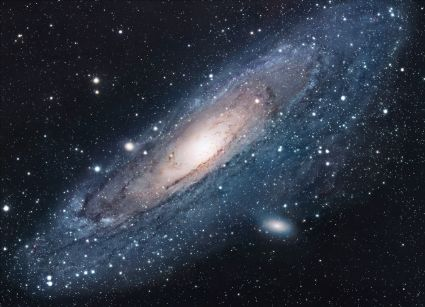
\includegraphics[scale=1.7]{universe}
\caption{The Universe}
\label{fig:universe}
\end{figure}

\end{comment}

\section{Conclusion}
Hector:
Aprendí bastante con este trabajo, aprendí las bases de la inteligencia artificial así como la implementación que esta tiene gracias a este proyecto. Aún hay mucho que aprender pero como alumno creo que tuve un gran crecimiento. Comprendí conceptos como onniciencia, además de comprender mejor los agentes racionales y identificarlos.

Daniel:
Aprendí las bases de la inteligencia artificial y el como este ha evolucionado hasta lo que hoy tenemos. Viendo desde ejemplos sencillos como saber si un agente es racional o no, y cuantos agentes hay en un istema, además de la implementación de dichos algoritmos.

Norman:
Este proyecto me ha servido para entender que la inteligencia artificial no es tan complicada como parece.
Tambien aprendi a pensar en soluciones optimas para implementar correctamente un algoritmo de busqueda de las mejores rutas, todo esto a traves de una enorme matriz con todo lo que implica 163 estaciones del metro para ser manejadas por Dijkstra, esto nos llevo a ingeniarnolas para crear esa matriz con ayuda de programas en C hechos por nosotros mismos, que nos facilitarian el trabajo unas 20 veces.
Otro punto importante es el manejo de programacion m en Matlab y uso de funciones para implementarlas en una GUI.

David: 
Fue una experiencia muy grata, el tener un acercamiento con los algoritmos de inteligencia artificial sin duda fue una excelente forma de implementar algo en matlab, aprendi a usar dijkstra y a usar los componentes basicos de una GUI en matlab, ademas de manejar matrices y vectores.
 \citep{}

\bibliographystyle{plain}
\bibliography{references}
\end{document}
